\documentclass{extbook}[14pt]
\usepackage{multicol, enumerate, enumitem, hyperref, color, soul, setspace, parskip, fancyhdr, amssymb, amsthm, amsmath, bbm, latexsym, units, mathtools}
\everymath{\displaystyle}
\usepackage[headsep=0.5cm,headheight=0cm, left=1 in,right= 1 in,top= 1 in,bottom= 1 in]{geometry}
\pagestyle{fancy}
\lhead{}
\chead{Answer Key for Module\,6\,-\,Polynomial\,Functions Version B}
\rhead{}
\lfoot{Summer\,C\,2020}
\cfoot{}
\rfoot{}
\begin{document}
\textbf{This key should allow you to understand why you choose the option you did (beyond just getting a question right or wrong). \href{https://xronos.clas.ufl.edu/mac1105spring2020/courseDescriptionAndMisc/Exams/LearningFromResults}{More instructions on how to use this key can be found here}.}

\textbf{If you have a suggestion to make the keys better, \href{https://forms.gle/CZkbZmPbC9XALEE88}{please fill out the short survey here}.}

\textit{Note: This key is auto-generated and may contain issues and/or errors. The keys are reviewed after each exam to ensure grading is done accurately. If there are issues (like duplicate options), they are noted in the offline gradebook. The keys are a work-in-progress to give students as many resources to improve as possible.}

\rule{\textwidth}{0.4pt}

26. Which of the following equations \textit{could} be of the graph presented below?
\begin{center} 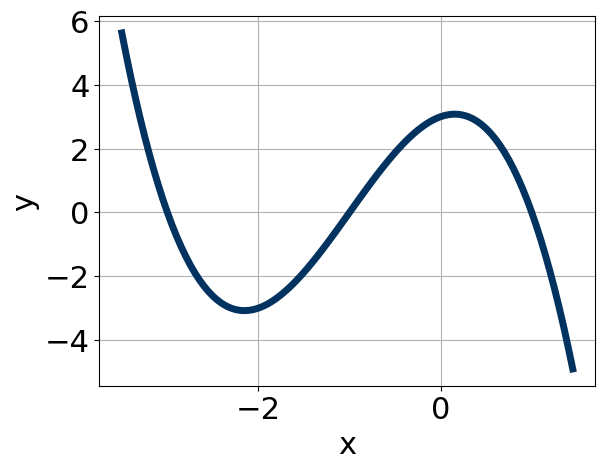
\includegraphics[width=0.3\textwidth]{../Figures/polyGraphToFunctionB.png} \end{center} 

The solution is $ -19x^{6} (x + 1)^{4} (x + 3)^{8} $ 

\begin{enumerate}[label=\Alph*.] 
\item $ -15x^{8} (x + 1)^{7} (x + 3)^{11} $ 

 The factors $(x + 1)$ and $(x + 3)$ should both have even powers. 
\item $ -19x^{6} (x + 1)^{4} (x + 3)^{8} $ 

 * This is the correct option. 
\item $ -8x^{6} (x + 1)^{4} (x + 3)^{5} $ 

 The factor $(x + 3)$ should have an even power. 
\item $ 8x^{10} (x + 1)^{6} (x + 3)^{7} $ 

 The factor $(x + 3)$ should have an even power and the leading coefficient should be the opposite sign. 
\item $ 4x^{6} (x + 1)^{4} (x + 3)^{8} $ 

 This corresponds to the leading coefficient being the opposite value than it should be. 
\end{enumerate} 
 
General Comments: Draw the x-axis to determine which zeros are touching (and so have even multiplicity) or cross (and have odd multiplicity).

-----------------------------------------------

27. Construct the lowest-degree polynomial given the zeros below. Then, choose the intervals that contain the coefficients of the polynomial in the form $ax^3+bx^2+cx+d$.
\[ \frac{-4}{5}, \frac{-3}{4}, \text{ and } \frac{-3}{5} \] 
The solution is $ 100x^{3} +215 x^{2} +153 x + 36 $ 

\begin{enumerate}[label=\Alph*.] 
\item $ a \in [91, 101], b \in [-217, -213], c \in [152, 155], \text{ and } d \in [-40, -29] $ 

 $100x^{3} -215 x^{2} +153 x -36$, which corresponds to multiplying out $(5x -4)(4x -3)(5x -3)$. 
\item $ a \in [91, 101], b \in [54, 60], c \in [-67, -59], \text{ and } d \in [-40, -29] $ 

 $100x^{3} +55 x^{2} -63 x -36$, which corresponds to multiplying out $(5x + 5)(4x -4)(5x -5)$. 
\item $ a \in [91, 101], b \in [213, 218], c \in [152, 155], \text{ and } d \in [33, 38] $ 

 * $100x^{3} +215 x^{2} +153 x + 36$, which is the correct option. 
\item $ a \in [91, 101], b \in [213, 218], c \in [152, 155], \text{ and } d \in [-40, -29] $ 

 $100x^{3} +215 x^{2} +153 x -36$, which corresponds to multiplying everything correctly except the constant term. 
\item $ a \in [91, 101], b \in [-103, -91], c \in [-36, -30], \text{ and } d \in [33, 38] $ 

 $100x^{3} -95 x^{2} -33 x + 36$, which corresponds to multiplying out $(5x + 5)(4x + 4)(5x -5)$. 
\end{enumerate} 
 
General Comments: To construct the lowest-degree polynomial, you want to multiply out $(5x + 4)(4x + 3)(5x + 3)$

-----------------------------------------------

28. Describe the end behavior of the polynomial below.
\[ f(x) = 8(x - 9)^{2}(x + 9)^{3}(x - 3)^{5}(x + 3)^{5} \] 

 
 The solution is  
 \begin{center} 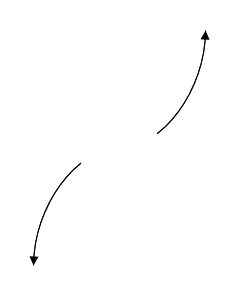
\includegraphics[width=0.3\textwidth]{../Figures/polyEndBehaviorDB.png} \end{center}\begin{tabular}{|c|c|} 
\hline 
 & \tabularnewline 
 \textbf{A.} 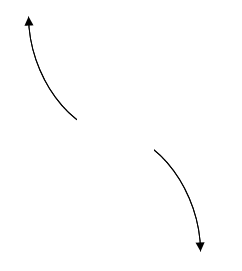
\includegraphics[width=0.3\textwidth]{../Figures/polyEndBehaviorAB.png} & \textbf{B.} 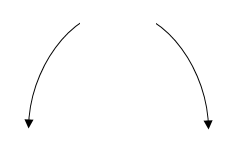
\includegraphics[width=0.3\textwidth]{../Figures/polyEndBehaviorBB.png} \tabularnewline 
\hline 
 & \tabularnewline 
 \textbf{C.} 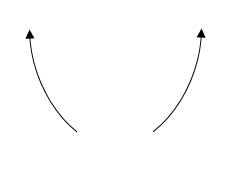
\includegraphics[width=0.3\textwidth]{../Figures/polyEndBehaviorCB.png} & \textbf{D.} 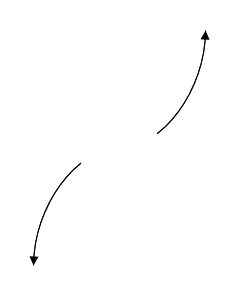
\includegraphics[width=0.3\textwidth]{../Figures/polyEndBehaviorDB.png} \tabularnewline 
\hline 
 E. None of the figures above. & \tabularnewline 
\hline 
 \end{tabular} 
 
\begin{enumerate}[label=\Alph*.] 
\item The function is above the $x$-axis, then passes through.  
\item The function is below the $x$-axis, then touches.  
\item The function is above the $x$-axis, then touches.  
\item The function is below the $x$-axis, then passes through.  
\end{enumerate} 
 
\textbf{General Comments:} Remember that end behavior is determined by the leading coefficient AND whether the \textbf{sum} of the multiplicities is positive or negative.

-----------------------------------------------

29. Construct the lowest-degree polynomial given the zeros below. Then, choose the intervals that contain the coefficients of the polynomial in the form $x^3+bx^2+cx+d$.
\[ -2 - 3i \text{ and } 4 \] 
The solution is $ x^{3} -3 x -52 $ 

\begin{enumerate}[label=\Alph*.] 
\item $ b \in [-0.55, 0.3], c \in [-3.37, -2.62], \text{ and } d \in [-55, -49] $ 

 * $x^{3} -3 x -52$, which is the correct option. 
\item $ b \in [0.39, 1.57], c \in [-1.54, -0.37], \text{ and } d \in [-21, -11] $ 

 $x^{3} + x^{2} -x -12$, which corresponds to multiplying out $(x + 3)(x -4)$. 
\item $ b \in [-0.55, 0.3], c \in [-3.37, -2.62], \text{ and } d \in [50, 54] $ 

 $x^{3} -3 x + 52$, which corresponds to multiplying out $(x-(-2 - 3i))(x-(-2 + 3i))(x + 4)$. 
\item $ b \in [0.39, 1.57], c \in [-2.16, -1.42], \text{ and } d \in [-11, -4] $ 

 $x^{3} + x^{2} -2 x -8$, which corresponds to multiplying out $(x + 2)(x -4)$. 
\item $ \text{None of the above.} $ 

 This corresponds to making an unanticipated error or not understanding how to use nonreal complex numbers to create the lowest-degree polynomial. If you chose this and are not sure what you did wrong, please contact the coordinator for help. 
\end{enumerate} 
 
General Comments: Remember that the conjugate of $a+bi$ is $a-bi$. Since these zeros always come in pairs, we need to multiply out $(x-(-2 - 3i))(x-(-2 + 3i))(x-(4))$.

-----------------------------------------------

30. Describe the zero behavior of the zero $x = -8$ of the polynomial below.
\[ f(x) = 4(x + 5)^{6}(x - 5)^{2}(x - 8)^{7}(x + 8)^{6} \] 

 
 The solution is  
 \begin{center} 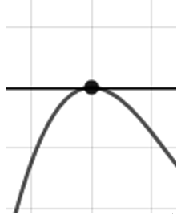
\includegraphics[width=0.3\textwidth]{../Figures/polyZeroBehaviorBB.png} \end{center}\begin{tabular}{|c|c|} 
\hline 
 & \tabularnewline 
 \textbf{A.} 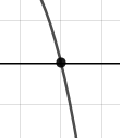
\includegraphics[width=0.3\textwidth]{../Figures/polyZeroBehaviorAB.png} & \textbf{B.} 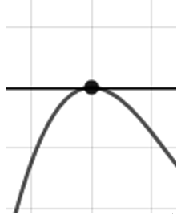
\includegraphics[width=0.3\textwidth]{../Figures/polyZeroBehaviorBB.png} \tabularnewline 
\hline 
 & \tabularnewline 
 \textbf{C.} 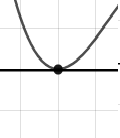
\includegraphics[width=0.3\textwidth]{../Figures/polyZeroBehaviorCB.png} & \textbf{D.} 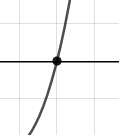
\includegraphics[width=0.3\textwidth]{../Figures/polyZeroBehaviorDB.png} \tabularnewline 
\hline 
 E. None of the figures above. & \tabularnewline 
\hline 
 \end{tabular} 
 
\begin{enumerate}[label=\Alph*.] 
\item   
\item   
\item   
\item   
\end{enumerate} 
 
\textbf{General Comments:} You will need to sketch the entire graph, then zoom in on the zero the question asks about.

-----------------------------------------------


\end{document}

